\documentclass[11pt, titlepage]{article} 

\usepackage{geometry}
\geometry{left=0.8in, right=0.8in, top=0.8in, bottom=0.8in}

\usepackage{color}
\usepackage{graphicx} % slike
\usepackage{caption}
\usepackage{subcaption}
\usepackage{siunitx} % enote
\usepackage{amsmath} % enačbe
\usepackage{amssymb} % simboli
\usepackage[thinc]{esdiff} % za odvode
\usepackage[colorlinks=true]{hyperref} % za linke
\usepackage{float} % za fiksiranje figur
\usepackage{mathtools}
\usepackage{esint} % za fancy integrale
\usepackage[numbib,nottoc]{tocbibind}
\usepackage[slovene]{babel}


\usepackage{tikz}

\newcommand{\dif}[1]{\,{\rm d}#1}

\begin{document}

\begin{titlepage}
    \begin{center}
        \includegraphics[width=0.5\textwidth]{figures/FRI_logo.png}\\
        \vspace{0.5cm}
        \vspace{3cm}
        {\LARGE \bf Sila težnosti} \\
        \vspace{0.3cm}
        \vspace{2.0cm}
        {\large Numerična matematika}\\
        \vspace{0.2cm}
        {|}\\
        \vspace{0.2cm}
        {\large 2. domača naloga}\\
        \vspace{2.0cm}
    \end{center}
    \vfill
    \begin{flushleft}
        {\normalsize {\sf Avtor:} Vito Levstik\\}
    \end{flushleft}
    \vspace{2cm}
    \begin{center}
        {\normalsize \sc Akademsko leto 2024/2025}
    \end{center}
\end{titlepage}

\newpage

\section{Uvod}

Cilj naloge je izračunati silo težnosti med dvema vzporednima homogenima enotskima kockama, na medsebojni razdalji $1$ (med najbljižjima stranicama) na 10 decimalk (z relativno natančnostjo $10^{-10}$). Predpostavimo, da so vse fizikalne konstante enake 1, kar pomeni, da je iskana sila
$$
\mathbf{F} = \int_{T_1} \int_{T_2} \frac{\mathbf{r}_1 - \mathbf{r}_2}{\left\lVert \mathbf{r}_1 - \mathbf{r}_2 \right\rVert_2^3} \, d\mathbf{r}_1 \, d\mathbf{r}_2
$$
kjer sta $T_1$ in $T_2$ kocki po katerih integriramo.

\section{Implementacija}
Najprej postavimo kocki v koordinatni sistem. Prva kocka $T_1$ naj bo $[0, 1]^3$, druga kocka $T_2$ pa $[2,3] \times [0,1]^2$. S tem zagotovimo, da sta kocki enotski, vzporedni in na razdalji 1. Sedaj lahko iskani integral zapišemo po komponentah
$$
\mathbf{F} = \int_{0}^{1} \int_{0}^{1} \int_{0}^{1} \int_{2}^{3} \int_{0}^{1} \int_{0}^{1} \frac{(x_1 - x_2, y_1 - y_2, z_1 - z_2)}{\left((x_1 - x_2)^2 + (y_1 - y_2)^2 + (z_1 - z_2)^2\right)^{3/2}} \, dz_2 \, dy_2 \, dx_2 \, dz_1 \, dy_1 \, dx_1,
$$
kjer so $(x_1, y_1, z_1)$ koordinate točk prve kocke in $(x_2, y_2, z_2)$ koordinate točk druge kocke.

Integral rešimo s Simpsonovo metodo. Ker imamo 6 integralov, bo naivna implementacija imela časovno kompleksnost $O(n^6)$, kjer je $n$ število delitev integracijskega intervala. Ker potrebujemo veliko natančnost, je tak naiven pristop nemogoč.
Ključna pohitritev je, da prevedemo 6-kratni integral v 3-kratnega, s čimer bomo spremenili časovno odvisnost v $O(n^3)$. Definiramo
$$
K(\mathbf{r}) = \frac{\mathbf{r}}{\left\lVert \mathbf{r} \right\rVert_2^3} 
\quad 
\text{ in } 
\quad 
\chi_T(\mathbf{r}) = \begin{cases}
    1 & \text{če } \mathbf{r} \in T \\
    0 & \text{drugače}
\end{cases}
$$
in tako zapišemo integral kot
$$
\mathbf{F} = \int_{\mathbb{R}^3} \int_{\mathbb{R}^3} K(\mathbf{r_1 - r_2}) \, \chi_{T_1}(\mathbf{r_1}) \, \chi_{T_2}(\mathbf{r_2}) \, d\mathbf{r_1}d\mathbf{r_2}
$$
Sedaj uvedemo novo spremenljivko $\mathbf{r} = (x,y,z) = \mathbf{r_1} - \mathbf{r_2}$. Ob upoševanju domen za $\mathbf{r_1}$ in $\mathbf{r_2}$ je $x \in [-3,-1]$, $y \in [-1,1]$ in $z \in [-1,1]$. Jakovijeva matrika je $-I_3$, kjer je $I_3$ enotska matrika v treh dimenzijah, zato je determinanta enaka $-1$. Iz tega sledi $d\mathbf{r_2} = |\text{det} J| \, d\mathbf{r} = d\mathbf{r}$, torej lahko pišemo
$$
\mathbf{F} = \int_{\mathbb{R}^3} \chi_{T_1}(\mathbf{r_1}) \int_{\mathbb{R}^3} \chi_{T_2}(\mathbf{r_1} - \mathbf{r}) K(\mathbf{r}) \, d\mathbf{r} \, d\mathbf{r_1}.
$$
Vrstni red integracije lahko zamenjamo in upoštevamo
$$
\chi_{T_2}(\mathbf{r_1} - \mathbf{r}) = 
\begin{cases}
    1 & \text{če } \mathbf{r_1} - \mathbf{r} \in T_2 \\
    0 & \text{drugače}
\end{cases}
=
\begin{cases}
    1 & \text{če } \mathbf{r_1} \in T_2 + \mathbf{r} \\
    0 & \text{drugače}
\end{cases}
=
\chi_{T_2 + \mathbf{r}}(\mathbf{r_1}).
$$
Tako dobimo
$$
\mathbf{F} = \int_{\mathbb{R}^3} K(\mathbf{r}) \int_{\mathbb{R}^3} \chi_{T_1}(\mathbf{r_1}) \, \chi_{T_2 + \mathbf{r}}(\mathbf{r_1}) \, d\mathbf{r_1} \, d\mathbf{r}.
$$
Pomemben razmislek je, da je notranji integral enak volumnu preseka kock $T_1$ in $T_2 + \mathbf{r}$, ki ga označimo z $V(\mathbf{r})$. Končen integral je tako
$$
\mathbf{F} = \int_{\mathbb{R}^3} K(\mathbf{r}) \, V(\mathbf{r}) \, d\mathbf{r}.
$$
Ker je presek dveh kock kvader, lahko $V(\mathbf{r})$ izračunamo kot produkt presekov po posameznih koordinatah. Ob upoštevanju domen za $\mathbf{r}$ dobimo
$$
V(x,y,z) = \left(\text{min}(1,3+x) - \text{max}(0,2+x)\right)(1+|y|)(1+|z|).
$$
Upoštevmo še dejstvo, da bo končna sila le v $x$ smeri, saj sta kocki vzporedni. Silo lahko tako zapišemo kot
$$
F_x = \int_{-3}^{-1} \int_{-1}^{1} \int_{-1}^{1} \frac{x}{\left(x^2+y^2+z^2\right)^{3/2}} \, V(x,y,z) \, dz \, dy \, dx,
$$
kar nam da časovno kompleksnost $O(n^3)$. Kompleksnost lahko še dodatno zmanjšamo na $O(n^2)$, če analitično izračunamo integral po $z$. Potrebno je overdnotiti
$$
\int_{-1}^{1} \frac{1-|z|}{\left(x^2+y^2+z^2\right)^{3/2}} \, dz.
$$
Ker je integrand soda funkcija, lahko integriramo na intervalu $[0,1]$ in rezultat pomnožimo z 2 (ter uporabimo $|z| = z$). Integral je tako
$$
2\int_{0}^{1} \frac{1}{\left(x^2+y^2+z^2\right)^{3/2}} \, dz - 2\int_{0}^{1} \frac{z}{\left(x^2+y^2+z^2\right)^{3/2}} \, dz.
$$
Pogledamo v tabele integralov \cite{Bronštejn_Semendjaev_1984}, izračunamo in dobimo
$$
\frac{2}{(x^2+y^2)\sqrt{x^2+y^2+1}} - \frac{2}{\sqrt{x^2+y^2}} + \frac{2}{\sqrt{x^2+y^2+1}} = f(x,y).
$$
Označimo $l(x) = \left(\text{min}(1,3+x) - \text{max}(0,2+x)\right)$. Končen integral je tako
$$
F_x = \int_{-3}^{-1} \int_{-1}^{1} x \, l(x) (1-|y|) f(x,y) \, dy \, dx.
$$

Sedaj implementiramo funkcijo \texttt{simpson2D(n)}, ki sprejme število delitev $n$ (mora biti sodo za Simpsonovo metodo) in vrne silo v $x$ smeri. Ker je širina integracijskih intervalov v $x$ in $y$ enaka $2$, uporabimo enako velikost koraka $h = 2/n$ za obe smeri.
V funkciji ustvarimo vektor uteži $w = [1, 4, 2, \ldots, 2, 4, 1]$, dolžine $n+1$, da lahko do iskanih uteži pri posameznih vozlih dostopamo s pomočjo indeksa. Funkcija je nato dvojna zanka po $x$ in $y$ koordinatah, kjer v zanki po $y$ iteriramo do polovice $n/2$ in nato pomnožimo rezultat z 2, saj je integrand soda funkcija v $y$ smeri. 
Za vsako točko $(x,y)$ izračunamo vrednost integranda, ga pomnožimo z utežjo in dodamo k skupni vsoti sile. Na koncu pomnožimo vsoto s faktorjem $h^2/9$, kar nam da končno vrednost sile v $x$ smeri.

Tekom postopka implementacije funkcije \texttt{simpson2D(n)} smo implementirali funkcije \texttt{simpson6D(n)}, ki je naivna implementacija 6-kratnega integrala, \texttt{simpson3D(n)}, ki je implementacija 3-kratnega integrala in \texttt{monte\_carlo\_integration(n)}, ki izračuna 6-kratni integral z Monte Carlo metodo.
Te funkcije smo implementirali, saj smo sprva mislili, da bo ne bo potrebna redukcija 6-kratnega integrala v 3-kratnega in 2-kratnega. Sedaj te funkcije lahko uporabimo za primerjavo rezultatov.

\section{Rezultati}
Da dosežemo željeno natančnost, povečujemo $n$ in preverimo da je absolutna vrednost kvocienta razlike med dvema zaporednima izračunoma in vrednosti zadnjega izračuna manjša od $10^{-10}$. Pri $n=200000$ dobimo silo, zaokroženo na 10 decimalk, $F\approx-0.2479229692$. Minus označuje, da je sila med kockama privlačna.
Pri tem je relativna natančnost $6.76 \cdot 10^{-11}$, kar je manj kot $10^{-10}$, zato lahko rezultat sprejmemo. Čas izvajanja je bil približno $1500$ sekund.

\begin{figure}[H]
    \centering
    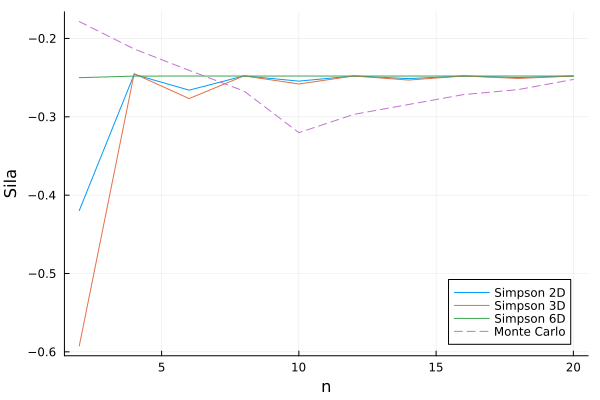
\includegraphics[width=0.75\textwidth]{figures/force_convergence.png}
    \caption{Konvergenca različnih metod.}
    \label{fig:convergence}
\end{figure}
Za konec še primerjamo konvergenco in časovno zahtevnost rezultatov različnih metod na različnih intervalih za $n$. Na sliki \ref{fig:convergence} so prikazane vrednosti sile za različne $n$.
Kljub temu, da je metoda \texttt{simpson6D} najpočasnejša, izgleda, da ima najboljšo konvergenco. \texttt{simpson3D} in \texttt{simpson2D} imata bistveno večja odstopanja pri $n=2,6,10,14,18$, kar je verjetno posledica tega, da zaradi preoblikovanja rešujemo drugačen integral kot na začetku. Ima pa \texttt{simpson2D} boljše rezultate kot \texttt{simpson3D}, kar je pričakovano,
saj je integral po $z$ že bil izračunan analitično. \texttt{monte\_carlo\_integration} je najslabša metoda, saj je nedeterministična in je odvisna od naključne izbire točk.

\begin{figure}[H]
    \centering
    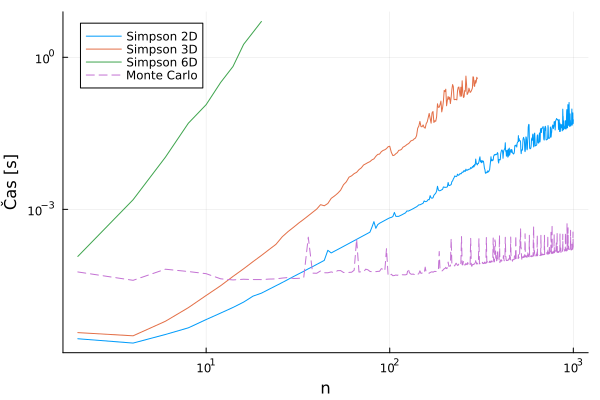
\includegraphics[width=0.75\textwidth]{figures/force_time.png}
    \caption{Čas izvajanja različnih metod.}
    \label{fig:time}
\end{figure}

Na sliki \ref{fig:time} so prikazani časi izvajanja različnih metod. Pričakovano je \texttt{simpson6D(n)} najpočasnejša. Metoda \texttt{simpson3D(n)} je bistveno hitrejša, vendar je \texttt{simpson2D(n)} najhitrejša od determinističnih metod. Metoda \texttt{monte\_carlo\_integration(n)} je hitrejša od vseh, kar je pričakovano, saj je potrebno izračunati le $n$ naključnih točk in izračunati povprečno vrednost integranda, torej ima časovno kompleksnost $O(n)$.
Ker pa je ta metoda nedeterministična, v nalogi pa iščemo natančno vrednost na 10 decimalk, te metode nismo uporabili. Če bi zadoščalo podati rezultat na 10 decimalk natančno z intervalom zaupanja, bi morda uporabili to metodo, odvisno od tega kako velik interval zaupanja bi želeli.


\bibliographystyle{unsrt}   % You can use other styles like alpha, ieeetr, apalike, etc.
\bibliography{references}   % Don't include the .bib extension

\end{document}